\section{Environment}

\subsection{Terminal and Basic Commands}
\begin{frame}{Terminal}
    \begin{block}{Opening Terminal}
        Open a terminal window by pressing \textbf{Ctrl+Alt+T}
    \end{block}
    \begin{figure}
        \centering
        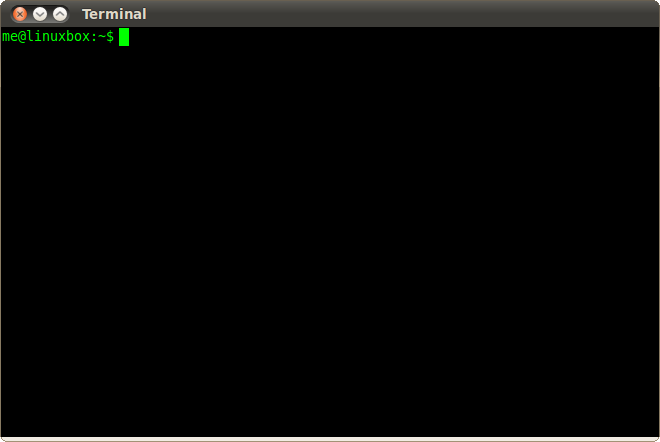
\includegraphics[width=\textwidth]{images/terminal.png}
    \end{figure}
\end{frame}

\begin{frame}{Directory Structure}
    \begin{figure}
        \centering
        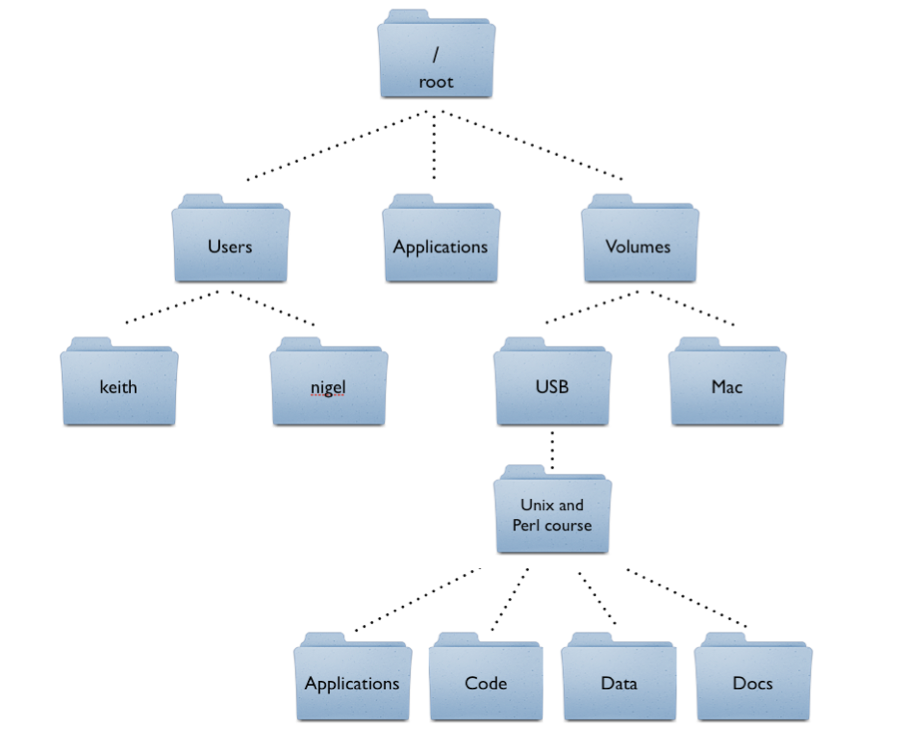
\includegraphics[height=0.7\textheight]{images/directory_tree.png}
    \end{figure}
\end{frame}

\begin{frame}[fragile]{Terminal Navigation}
    \begin{itemize}
        \item Type a command in the terminal, and press \textbf{Enter}
        \item Make a new directory (folder) --
            \begin{minted}{bash}
                mkdir <directory_name>
            \end{minted}
        \item Enter a directory --
            \begin{minted}{bash}
                cd <directory_name>
            \end{minted}
        \item List contents of directory --
            \begin{minted}{bash}
                ls
            \end{minted}
    \end{itemize}
\end{frame}

\subsection{Editor}
\begin{frame}[fragile]{Text Editor}
    \begin{itemize}
        \item Write your code in a text editor
            \begin{itemize}
                \item Notepad, Vim, Emacs, etc.
            \end{itemize}
        \pause
        \item We will use \textbf{gedit}
        \pause
        \item Open \emph{gedit}
            \begin{minted}{bash}
                gedit &
            \end{minted}
        \item Open a file with \emph{gedit}
            \begin{minted}{bash}
                gedit my_file.cpp &
            \end{minted}
            \pause
            \begin{itemize}
                \item Note that the file should be present in your current directory
                \item If file doesn't exist, it will be created
            \end{itemize}
    \end{itemize}
\end{frame}
